\documentclass[tikz,convert={density=150,size=600,outext=.png}]{standalone}
\usetikzlibrary{shapes, calc, arrows, fit, positioning, decorations, patterns, decorations.pathreplacing, chains, snakes}

\begin{document}
% The first pyramid, three steps
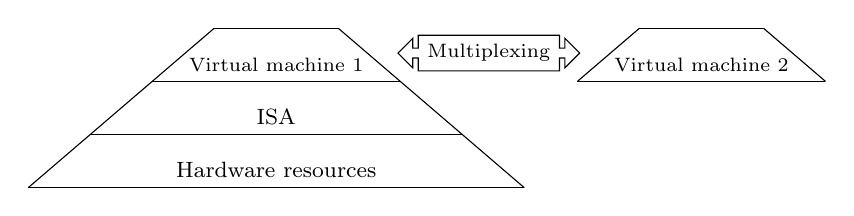
\begin{tikzpicture}[scale=0.9]
\coordinate (A) at (-3.5,-3) {};
\coordinate (B) at ( 3.5,-3) {};
\coordinate (C) at ( 0, 0) {};
\draw (A) -- ($(A)!3/4!(C)$);
\draw (B) -- ($(B)!3/4!(C)$);
\draw ($(A)!3/4!(C)$) -- ($(B)!3/4!(C)$);
    \foreach \y/\A in {0/{Hardware resources},
                       1/{ISA},
                       2/{\scriptsize Virtual machine 1}
                       } {
        \draw ($(A)!\y/4!(C)$) -- ($(B)!\y/4!(C)$)
        node[midway,above] {\footnotesize\A};
    };

% The second pyramid, only one step
% Copy-pasted from the first one and shifted
\coordinate (D) at (6-3.5,-3) {};
\coordinate (E) at (6+3.5,-3) {};
\coordinate (F) at (6,     0) {};
\draw ($(D)!2/4!(F)$) -- ($(D)!3/4!(F)$);
\draw ($(E)!2/4!(F)$) -- ($(E)!3/4!(F)$);
\draw ($(D)!3/4!(F)$) -- ($(E)!3/4!(F)$);
    \foreach \y/\A in {2/{\scriptsize Virtual machine 2}
                       } {
        \draw ($(D)!\y/4!(F)$) -- ($(E)!\y/4!(F)$)
        node[midway,above] {\footnotesize\A};
    }

% The multiplexing "arrow"
\node [ arrow box, draw, arrow box arrows={east:.25cm, west:0.25cm}] at (3,-1.1) {\scriptsize Multiplexing};
\end{tikzpicture}
\end{document}
